\documentclass{article}

% Language setting
% Replace `english' with e.g. `spanish' to change the document language
\usepackage[english]{babel}

% Set page size and margins
% Replace `letterpaper' with`a4paper' for UK/EU standard size
\usepackage[letterpaper,top=2cm,bottom=2cm,left=3cm,right=3cm,marginparwidth=1.75cm]{geometry}

% Useful packages
\usepackage{amsmath}
\usepackage{graphicx}
\usepackage[colorlinks=true, allcolors=blue]{hyperref}
\usepackage{float}
\usepackage{amsthm}
\usepackage{graphicx}
\usepackage{amssymb}
\usepackage[dvipsnames]{xcolor}
\usepackage{verse}
\usepackage[demo]{graphicx}
\usepackage{subcaption}

\newtheorem{theorem}{Theorem}[section]
\newtheorem{corollary}{Corollary}[theorem]
\newtheorem{lemma}[theorem]{Lemma}

\theoremstyle{definition}
\newtheorem{definition}{Definition}[section]

\theoremstyle{remark}
\newtheorem*{remark}{\textbf{Remark}}

\theoremstyle{example}
\newtheorem{example}{\textbf{Example}}[section]

\newcommand{\attrib}[1]{%
\nopagebreak{\raggedleft\footnotesize #1\par}}
\renewcommand{\poemtitlefont}{\normalfont\large\itshape\centering}

\newcommand{\qedwhite}{\hfill \ensuremath{\Box}}

\title{Project Rough Draft}
\author{Ruiqi (Rickey) Huang}

\begin{document}
\maketitle

\section{Abstract}

\paragraph{  }

This project investigates the Stirling numbers of the first and second kind and their recurrence relations. The flow of the project is motivated by solving the problem of counting the rhyme scheme of a poem with a given number of lines and a given number of rhymes. The recurrence relations for the both kinds of Stirling numbers are proved combinatorially. In the end of the project two problem of counting rhyming scheme are explored and answered using what we prove about the Stirling numbers.

\section{Introduction}

\paragraph{   }

This project introduces the Stirling numbers of both the first kind and the second kind. The discussion of the Stirling numbers and their recurrence relations can be motivated by solving problems of partitioning a set into a restricted number of subsets. The main goal of this project is to understand the Stirling number of the first and second kinds and to prove their recurrence relations. At the later part of the project, one application of the Stirling numbers on counting the possible rhyme schemes of a fixed-line poem will be elaborated.

\subsection{Related Real World Problem \label{"rwProblems"}}
\paragraph{   }

Considering the problem of arranging a group of $n$ friends into $k$ smaller groups, and these groups can be any size from $1$ to $n$ but cannot be empty. The number of ways to find such subsets is the same as to find $k$ disjoint subsets from a set with $n$ labeled elements. This gives the chance to introduce the Stirling numbers of the second kind. Looking at the problem of arranging friends again, what if we want to not only divide $n$ friends into $k$ groups but also sit each group at a circular table (which means we need to decide who sit next to whom in a fixed direction, clockwise or counterclockwise). This can be converted to a problem of counting the number of possible $n$-permutations with $k$ cycles where a cycle is of size $1$ to $n$ \cite{bona_combinatorics_2012}. This is exactly what the Stirling number of the first kind counts.

\subsection{Motivating Problem: Rhyme Scheme}\label{sec:2.2}
\paragraph{  }

In English poems and songs, people using the rhymes to create a pleasure of reading and predicting the poems. The rhyme schemes are the pattern of rhymes located at the last word of each line. For example, in the poem "\textit{Stopping by Woods on a Snowy Evening}" written by Robert Frost (as shown below), He used the rhyme scheme AABA BBCB CCDC, where A represents the rhyming syllables "-ow" (or "-ough"); B represents the rhyming syllables "-ere" ("-eer", or "-ear"); C represents the rhyming syllables "-ake"; and D represent the rhyming syllables "-eep".

\poemtitle{Stopping by Woods on a Snowy Evening}
\settowidth{\versewidth}{His house is in the village though;}
\begin{verse}[\versewidth]
Whose woods these are I think I know.\\
His house is in the village though;\\
He will not see me stopping here\\
To watch his woods fill up with snow.\\
\\
My little horse must think it queer\\
To stop without a farmhouse near\\
Between the woods and frozen lake\\
The darkest evening of the year.\\
\\
He gives his harness bells a shake\\
To ask if there is some mistake.\\
The only other sound’s the sweep\\
Of easy wind and downy flake.
\end{verse}
\attrib{Robert Frost (1874--1963)}

To create a various unique poems and songs, poets and song writers would us a many different rhyme schemes in different works. Then, a question would be raised as following. How many rhyme schemes are there if we know how many lines and the number of rhymes we plan to write? Surprisingly, the Stirling numbers could help in this problem.

\subsection{Background Concepts}
\paragraph{   }

In order to have a clear understanding of the Stirling numbers and prove the recurrence relations of them, the background knowledge below should be first explained well to understand the details in the project.
\begin{itemize}
\item \textbf{Subsets:} When discussing the Stirling numbers in this paper, the subsets are considered to not include the empty subset.
\item \textbf{Partitions:} The partition of a set is a way to divide a set into disjoint subsets.
\item \textbf{Permutations:} A $n$-permutation $\sigma$ is a way to keep track of how elements are sent to other elements. The permutations in these project are denoted in the one-line cycle notation, such as $(1234)(56)(7)$ of a $7$-permutation means the following maps\cite{guichard_combinatorics_nodate}:

\begin{center}
$1 \mapsto 2$, $2 \mapsto 3 $, $3\mapsto 4$, $4\mapsto 1$\\
$5\mapsto 6$, $6\mapsto 5$\\
$7 \mapsto 7$
\end{center}

\item \textbf{Cycles and Cycle Types:} A cycle represents the number of parentheses in the cycle notation introduced above. For example $(1234)(56)(7)$ contains $3$ cycles. The cycle types keep track of the type of permutations, and sometimes the cycle that contains only one element would be omitted \cite{guichard_combinatorics_nodate}. For example, $(1234)(56)(7)$ (or $(1234)(56)$) is of $(3,2)$ cycle type.
\item \textbf{Falling and Rising Factorials:} Falling and rising factorials are used to prove the recurrence relation of the Stirling numbers algebraically. The falling factorials are defined as the product ${\displaystyle \prod_{k = 0}^{n - 1}{(x-k})}$ and denoted as $(x)_n$ or $x^{\underline{n}}$. In a similar way, the rising factorials are defined as the produce  ${\displaystyle \prod_{k = 0}^{n - 1}{(x+k})}$ and denoted as $x^{(n)}$ or $x^{\overline{n}}$\cite{bona_combinatorics_2012}.
\end{itemize}

\section{The Stirling number of the second kind ($s(n,k)$)}
\subsection{Definition}

\begin{definition}[\textbf{The Stirling number of the second kind}]\label{def:SN2nd}
    The Stirling number of the second kind is the number of ways to divide an $n$-object set into $k$ partitions, and it is always denoted as $s(n,k)$.
\end{definition}

Specially, $s(0,0) = 1$, since there is one partition for the empty set which is partition it into the empty set it self. This is the only case we consider the empty set as a subset. Also, $s(n,0) = 0, \; \forall n \in \mathbb{N^{+}}$, because there are no way to partition a nonempty set into $0$ subset. Similarly, $s(n,1) = 1, \; \forall n \in \mathbb{N^{+}}$, since there are only one way to partition a nonempty set into $1$ subset which is just itself. Finally, $s(n,n) = 1, \; \forall n \in \mathbb{N^{+}}$, because the only partition that divides a $n$-element set into $n$ subsets is that every element is in the subset only containing itself.

\begin{example}
    Considering the problem of arranging 4 friends into 2 groups. There are two possible ways to create the two groups: two groups with $3$ and $1$ people in them or two groups with $2$ and $2$ people in them. Hence suppose we label the friend with A, B, C, and D. There are $7$ ways to put them in to two groups:
        \begin{center}
        $\{A,B,C\}\bigcup \{D\},\; \{A,B,D\}\bigcup\{C\},\; \{A,C,D\}\bigcup\{B\},\; \{B,C,D\}\bigcup\{A\}$\\
        $\{A,B\}\bigcup\{C,D\},\; \{A,C\}\bigcup\{B,D\},\;\{A,D\}\bigcup\{B,C\}$
        \end{center}
\end{example}

\subsection{Recurrence Relation}
\begin{theorem}[\textbf{The recurrence relation for Stirling numbers of the second kind}]\label{thm:RR2nd}
    The Stirling numbers of the second kind follow a recurrence relation as the following:
    \begin{equation}\label{eqn:RR2nd}
        s(n+1,k) = s(n,k-1) + k\cdot s(n,k)
    \end{equation}
\end{theorem}

\begin{proof}[\textbf{proof}]
    We will finish a task of partitioning an $n+1$-element set $S_{n+1} = \{s_1, s_2, \cdots, s_{n+1}\}$ into $k$ subsets. Take $S_{n+1}$, we could think about which subset that $s_{n+1}$ falls into. 
    
    Considering the first possibility that it is in a subset that only contains itself. Then the question left is how to partition $S_n = \{s_1, s_2, \cdots, s_n\}$ into $k-1$ subsets. There are $s(n,k-1)$ ways to do the desired partition. 
    
    Then we can considering the second case that the element $s_{n+1}$ is in a subset that already have some other elements. Under this circumstance, we could first think about how to partition $S_{n}$ into $k$ subsets. There are $s(n,k)$ way to do the partition. Next, we want to put $s_{n+1}$ into one of these subsets, and because the order in the subsets are not considered by us, there are $k$ subsets can be chosen to put $s_{n+1}$.
    
    In this way, we obtain our recurrence relation in the equation (\ref{eqn:RR2nd}), where $s(n,k-1)$ is the number of way of partitions in the first case, and $k\cdot s(n,k)$.
\end{proof}

\section{\textbf{The Stirling number of the first kind ($c(n,k)$)}}
\subsection{Definition}

\begin{definition}[\textbf{The Stirling number of the first kind}]\label{def:SN1st}
    The Stirling number of the first kind is the number of $n$-permutations with $k$ cycles, denoted as $c(n,k)$.
\end{definition}

In order to get a desirable recurrence relation in the Section \ref{sec:4.2}, we set $c(0,0) = 1$, $c(n,0) = 0, \; \forall n \in \mathbb{N^{+}}$. With the similar reason as the Stirling number of the second kind in the Definition \ref{def:SN2nd}, and $c(n,n) = 1, \; \forall n \in \mathbb{N^{+}}$, but $c(n,1) \neq 1$, because in this one cycle, the order matters. In fact, $c(n,1) = (n-1)!,\; \forall n \in \mathbb{N^{+}}$ since after we fix the smallest entry to always be the first entry, we just need to permute the rest of the entries to get all of the permutations with one cycle.

\begin{example} \label{ex:c(4,2)}
Considering the problem of sitting $4$ friends at $2$ circular tables. Using the cycle notations, we can consider people in the same cycle as sitting at the same table. Under this circumstance, the permutations $(ABC)$ and $(ACB)$ are different arrangements. There are 11 ways in total to finish this task.

As shown in Figure \ref{vis:V1}, the $11$ ways to sit $4$ friend at $2$ round tables are visualized. The arrows in the drawings represent "next to". For example, $A \rightarrow B$ means A is sitting next to B.

\begin{figure}[H]
\centering
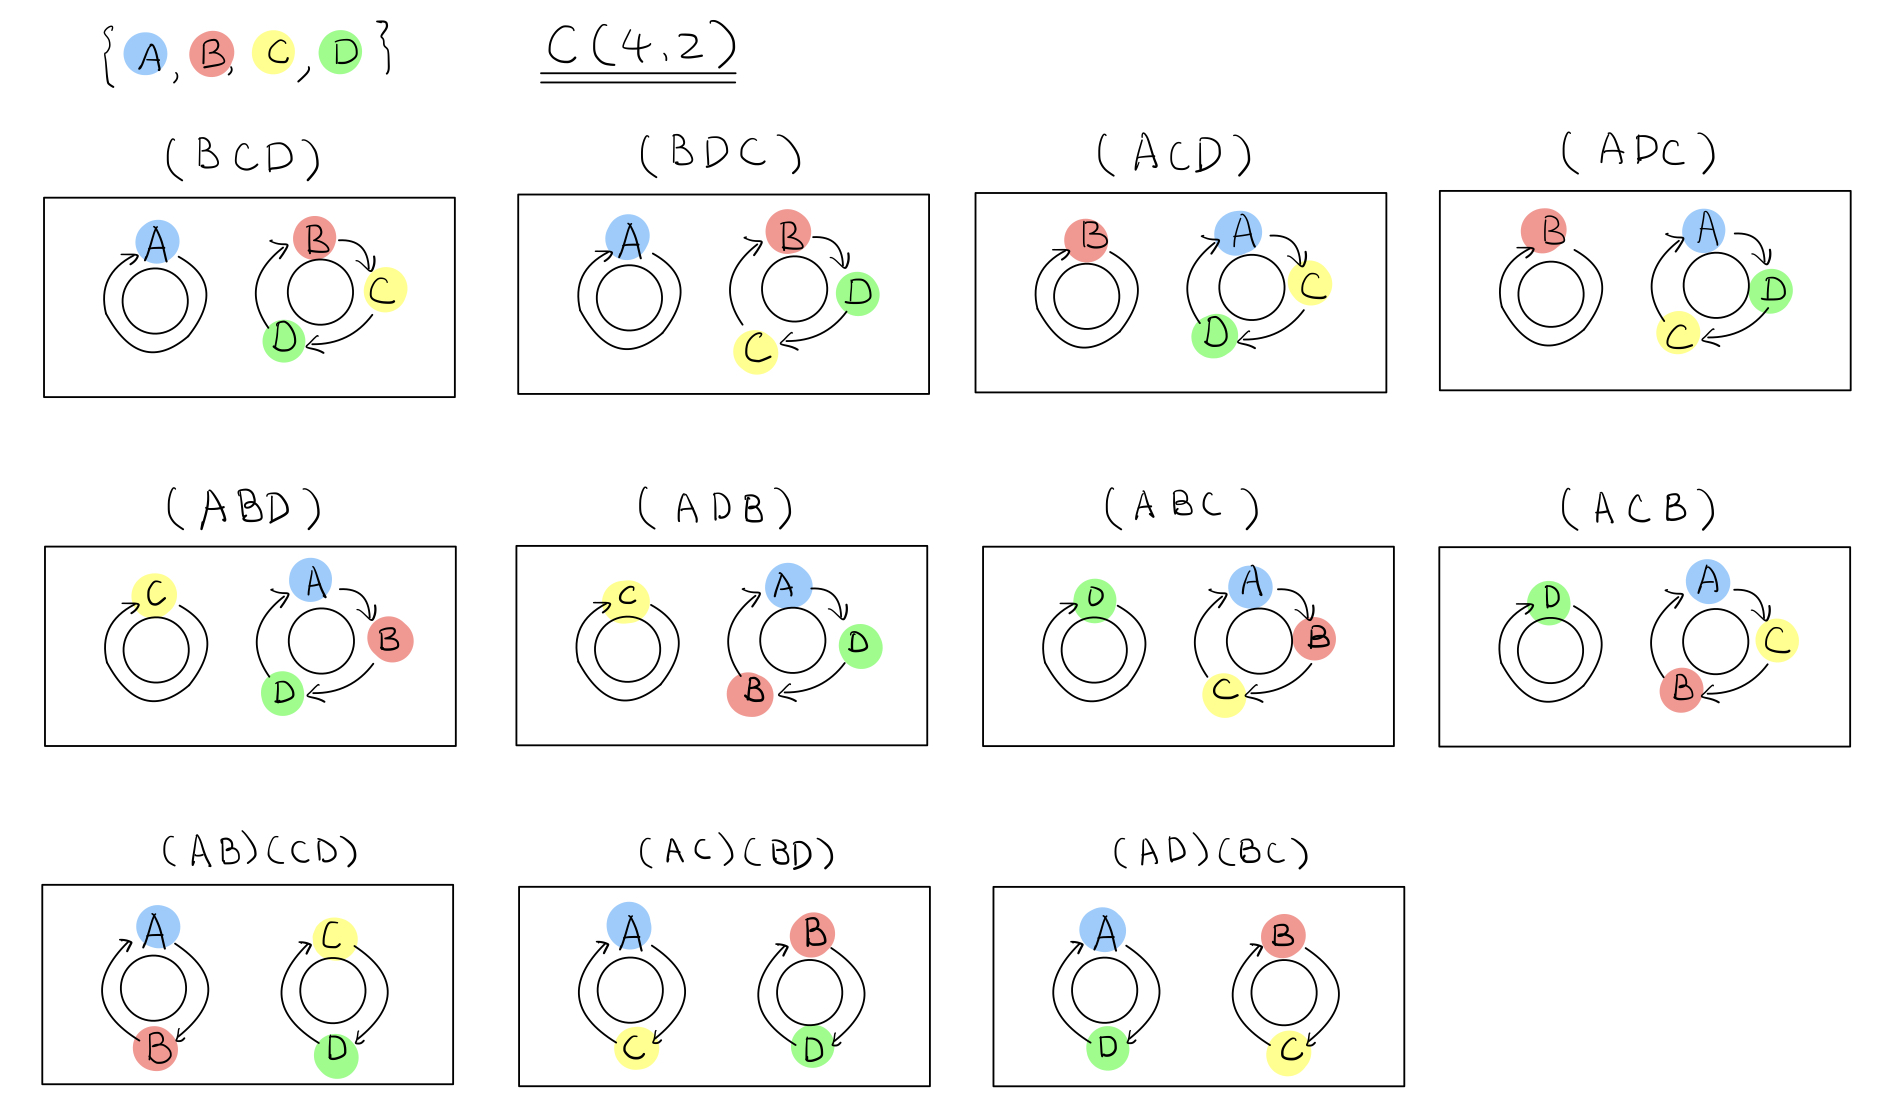
\includegraphics[width=0.6\textwidth]{Visualization1.jpeg}
\caption{\label{vis:V1}Visualization of $c(4,2)$}
\end{figure}
\end{example}

\subsection{Recurrence Relation}\label{sec:4.2}
\begin{theorem}[\textbf{The recurrence relation for Stirling numbers of the first kind}]\label{thm:RR1st}
    The Stirling numbers of the first kind follow a recurrence relation as the following:
    \begin{equation}\label{eqn:RR1st}
        c(n+1,k) = n\cdot c(n,k) + c(n,k-1)
    \end{equation}
\end{theorem}

\begin{proof}[\textbf{combinatorial proof}]\label{prf:RRpf1st}
    Consider an $n+1$-permutation $\sigma_{n+1}$ with $k$ cycles, it can be derived from two ways. The first situation is that $\sigma_{n+1}$ is obtained from adding one cycle that only contains $n+1$ to an $n$-permutation $\sigma_n$ with $k-1$ cycles. The other situation is that $\sigma_{n+1}$ is created by sticking $n+1$ into some position of one of the cycles in $\sigma_n$ with $k$ cycles.
    
    In the first case, the number of $\sigma_n$ with $k-1$ cycles is $c(n,k-1)$.
    
    In the second case, the number of $\sigma_n$ with $k$ cycles is $c(n,k)$. The rest of the task is to insert $n+1$ into such permutations. If we always insert $n+1$ after a certain entry in a certain cycle, we could create a new permutation $\sigma_{n+1}$ without creating a new cycle. We want to always inserting after an entry, because we want to make sure we include every permutations $\sigma_{n+1}$ created in this way. Hence there are $n$ ways in total to finish this step. Then, in total there are $n\cdot c(n,k)\; \sigma_{n+1}$ created in this way.
\end{proof}

\begin{example}
Considering the second step of the second case above, if we have a permutation $\sigma_5 = (123)(45)$ and want to create a permutation $\sigma_6$ follow the method in the proof, we would have the following permutations:
    \begin{center}
        $(1623)(45), \; (1263)(45), \; (1236)(45), \; (123)(465), \;(123)(456)$
    \end{center}
    $5$ permutations in total. 
\end{example}

\begin{remark}
    The reason why we don't want to consider $(6123)(45)$ and $(123)(645)$ in the previous example is that they are actually equivalent to permutations listed above. To be more specifically, $(6123)(45) = (1236)(45)$, and $(123)(645) = (123)(456)$.
\end{remark}

\begin{example}
    Considering again about the Example \ref{ex:c(4,2)}. Let $C_{(n,k)}$ denotes all the $n$-permutations that have $k$ cycles, such that $\lvert C_{(n,k)}\rvert = c(n,k)$. Then, following the proof \ref{prf:RRpf1st}, we could doing the first case by mapping elements in $C_{(3,1)}$ to elements in $C_{(4,2)}$. The detailed visualization for this mapping is shown in the Figure \ref{vis:V3}. In the second case, we first find elements in $C_{(3,2)}$ and then send each element of $C_{(3,2)}$ to $3$ distinct elements in $C_{(4,2)}$ by inserting the entry D after A, B, and C respectively. The visualization for this mapping is shown in the Figure \ref{vis:V2}.
    
    
    \begin{figure}[H]
        \centering
        \begin{minipage}{.5\textwidth}
            \centering
            \includegraphics[width=1\textwidth]{Visualization2.jpeg}
            \caption{\label{vis:V2}Visualization of mapping $C_{(3,2)}$ to $C_{(4,2)}$}
        \end{minipage}%
        \begin{minipage}{.5\textwidth}
            \centering
            \includegraphics[width=0.8\textwidth]{Visualization3.jpeg}
            \caption{\label{vis:V3}Visualization of mapping $C_{(3,1)}$ to $C_{(4,2)}$}
        \end{minipage}
    \end{figure}
\end{example}

\section{Applications of the Stirling numbers: Rhyme Scheme}
\paragraph{  }

Looking back to the motivating problem we mentioned in the Section \ref{sec:2.2}, we consider the question that if we fix the number of lines and the number of rhymes we plan to write, how many rhyme schemes are there can be written?

In order to connect solve this problem with the Stirling number of the first kind, we first need to figure out what is $n$ and $k$ in this problem. Since we know how many lines we plan to write, then there are $n$ lines that we can choose from. Also, because we are given the number of rhymes we want to compose, we could consider put lines with the same rhyming syllable into the same subset. Then we know what is corresponding to the number of subsets. Then, we could consider the following question.

\begin{example}

Considering the poem "\textit{Stopping by Woods on a Snowy Evening}" mentioned in the Section \ref{sec:2.2}, suppose before Robert Frost had wrote this poem he had decided he would use $3$ rhyming syllables to write the first two stanzas of the poem, but he haven't decide which rhyme scheme he would like to choose to write the poem. What is the probability that he actually wrote the one that is well-known nowadays?
\end{example}

\paragraph{  }

By the given, we know that Frost will use $8$ lines to create $3$-rhyme stanzas. Then, it is the problem of regrouping $8$ lines into $3$ groups, where each group is using one unique rhyming syllables. This is exactly what the Stirling number of the second kind counts (number of $4$-subset partitions of a set with $12$ elements). Then the total number of possible poems is $s(8,3)$ \cite{pollard_c_2003}.

Then, we would use the recurrence relation in the equation (\ref{eqn:RR2nd}) recursively to compute the exact number for $s(8,3)$:

\begin{align}
    s(8,3) &= s(7,2) + 3s(7,3)\\
    & = (s(6,1) + 2s(6,2)) + 3(s(6,2) + s(6,3))\\
    & = (1 + 2(s(5,1) + 2s(5,2))) + 3((s(5,1) + 2s(5,2)) + (s(5,2) + 3s(5,3)))\\
    & = (1 + 2(1 + 2(s(4,1) + 2s(4,2)))) + 3((1 + 2(s(4,1) + 2s(4,2))) \\
    & + ((s(4,1) + 2s(4,2)) + 3(s(4,2) + 3s(4,3))))\\
    & = (1 + 2(1 + 2(1 + 2(s(3,1) + 2s(3,2))))) + 3((1 + 2(1 + 2(s(3,1) + 2s(3,2)))) \\
    & + ((1 + 2(s(3,1) + 2s(3,2))) + 3(s(s(3,1) + 2s(3,2)) + 3(s(3,2) + 3s(3,3)))))\\
    & = (1 + 2(1 + 2(1 + 2(1 + 2(s(2,1) + 2s(2,2)))))) \\
    & + 3((1 + 2(1 + 2(1 + 2(s(2,1) + 2s(2,2))))) + ((1 + 2(1 + 2(s(2,1) \\
    &+ 2s(2,2)))) + 3(s(1 + 2(s(2,1) + 2s(2,2))) + 3((s(2,1) + 2s(2,2)) + 3))))\\
    & = (1 + 2(1 + 2(1 + 2(1 + 2(1 + 2))))) + 3((1 + 2(1 + 2(1 + 2(1 + 2)))) \\
    & + ((1 + 2(1 + 2(1 + 2))) + 3((1 + 2(1 + 2)) + 3((1 + 2) + 3))))\\
    & = (1 + 2(1 + 2(1 + 2(1 + 6)))) + 3((1 + 2(1 + 2(1 + 6))) \\
    & + ((1 + 2(1 + 6)) + 3((1 + 6) + 3(3 + 3))))\\
    & = (1 + 2(1 + 2(1 + 14))) + 3((1 + 2(1 + 14)) + ((1 + 14) \\
    & + 3((7 + 18)))\\
    & = (1 + 2(1 + 30)) + 3((1 + 30) + (15 + 3(25))\\
    & = (1 + 62) + 3(31 + 90)\\
    & = 63 + 363\\
    & = 426
\end{align}

Hence, the probability that Frost wrote the first two stanzas of "\textit{Stopping by Woods on a Snowy Evening}" under the situation the problem given is $\tfrac{1}{426} \approx 0.00235$.\qedwhite

\paragraph{  }

Similarly, the Stirling number of the first kind can also be used to solve some rhyme scheme problems.

\begin{example}
    Suppose a poet want to write a short poem with $5$ lines using $2$ rhymes, and the poet has already come up with two lines with distinct rhyming syllables, say "-eep" and "-ood". Also, he wants these two lines be the first line among the lines using the same rhyming syllables. How many poems he can write then?
\end{example}

\paragraph{  }

In this problem, more than just fixing the number of lines and rhymes, we also fix the first line of each group of rhyming syllable. This is actually the number of $5$-permutations with $2$ cycles, because when we decide how each cycle looks like, we fixed on entry in the cycle and permute the rest. Then, the problem is asking what is the value of $c(5,2)$ \cite{rogers_rhyming_1981}.

In order to compute $c(5,2)$, we need to use the recurrence relation in the equation (\ref{eqn:RR1st}) recursively:

\begin{align}
    c(5,2) & = 5c(4,2) + c(4,1)\\
    & = 5(11) + (4-1)!\\
    & = 55 + 3!\\
    & = 55 + 6\\
    & = 61
\end{align}

Hence, there are 61 possible poems he can write under the given requirement. \qedwhite

\newpage
\bibliography{sources}
\bibliographystyle{alpha}
\nocite{*}

\end{document}